\documentclass[12pt, UTF8, a4paper]{ctexart}
\usepackage{morelull}
\usepackage{graphicx}
\usepackage{booktabs}
\usepackage{threeparttable}

\title{中文长文本情感分类\ 实验报告}
\author{2018011365 张鹤潇}
\date{\today}

\begin{document}

\begin{titlepage}
    
\maketitle

\tableofcontents

\thispagestyle{empty}
\end{titlepage}

\setcounter{page}{1}

\section{研究背景}

情感分类是NLP领域的基本问题之一。
本次分类实验使用的数据源于新浪中文新闻,
根据网民对新闻的情感投票确定新闻标签。

具体而言,对每条新闻,取其获得票数最多的一类情感作为标签。
如果某新闻得票最多的情感有多个,就将其舍弃。
原始语料中包含链接、电话号等无关信息,我通过预处理将这些噪声筛去,
并从测试集中划分出一半作为验证集。

\begin{table}[htbp]
    \centering
    \caption{\label{tab:1} 数据类别分布}
    \begin{tabular}{cccccccccc}
    \toprule 
        类别 & 感动 & 同情 & 无聊 & 愤怒 & 搞笑 & 难过 & 新奇 & 温馨 & 总计 \\
        \midrule 
        训练集 & 366 & 81 & 104 & 912 & 344 & 178 & 95 & 27 & 2107 \\
        验证集 & 146 & 29 & 30 & 499 & 176 & 83 & 27 & 7 & 997 \\
        测试集 & 149 & 28 & 41 & 472 & 154 & 90 & 39 & 4 & 997 \\
        \bottomrule 
    \end{tabular}
\end{table}

该数据集具样本量小、类别分布极不均衡、
样本标注不准确、测试集与训练集不同分布等问题。在这种数据集上做情感分类的挑战非常大。

\section{模型介绍}

\subsection{Naive Bayes, SVM和random forest}

用Naive Bayes,SVM和random forest三种机器学习方法作对比实验,
其中SVM和random forest使用tf-idf特征。因SVM使用的hinge loss不支持输出概率,
故无法计算相关系数。

\subsection{MLP}

由两层全连接层构成的模型,特点是参数量大,易过拟合。
在全连接层间加入了Batch Normalization以提高性能。

\subsection{fastText}

fastText
\footnote{\href{https://arxiv.org/pdf/1607.01759.pdf}
{[Bag of Tricks for Efficient Text Classification, 2016]}}
是一种简洁有效的文本分类模型,其思路是
将所有词向量的均值作为文本的特征表示。
这里的词向量不仅来源于文本的unigram,还可以来源于bigram,trigram等。
fastText将N-gram融入特征中,
并用哈希解决组合爆炸的问题。

fastText也是训练词向量的方法之一。

\begin{figure}[htb]
    \centering
    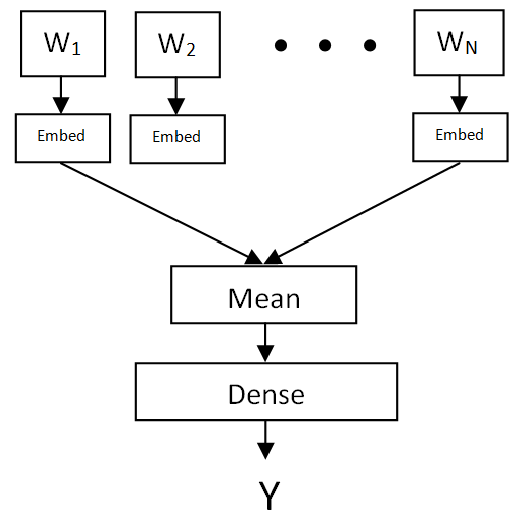
\includegraphics[width=2in, keepaspectratio]{./pic/fastText.png}\\
    \caption{fastText结构图}
\end{figure}

\subsection{TextCNN}

TextCNN
\footnote{\href{https://arxiv.org/abs/1408.5882}
{[Convolutional Neural Networks for Sentence Classification, 2014]}}
通过对词向量序列的卷积操作
提取文本的N-gram特征,沿着每个卷积核的输出做max pooling,
用dropout防止全连接层过拟合。

\begin{figure}[htb]
    \centering
    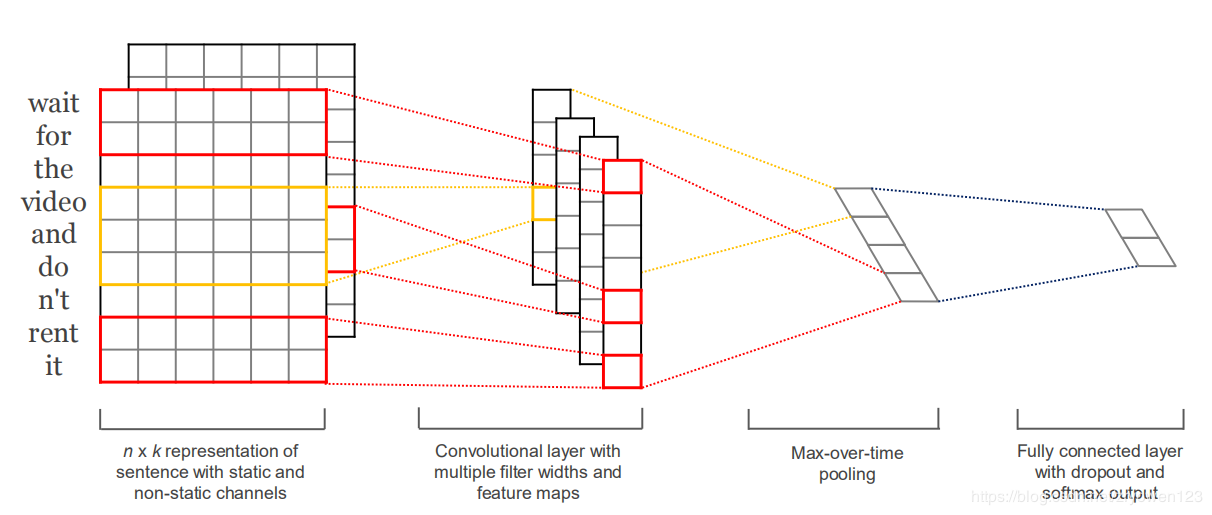
\includegraphics[width=5in, keepaspectratio]{./pic/cnn.png}\\
    \caption{TextCNN结构图}
\end{figure}

\subsection{Deep Pyramid CNN}

卷积层能有效提取局部的语义信息,但不擅长提取全局特征,
为了解决这个问题,就要增加网络的深度。

Deep Pyramid CNN
\footnote{\href{https://www.aclweb.org/anthology/P17-1052.pdf}
{[Deep Pyramid Convolutional Neural Networks for Text Categorization, 2017]}}
在TextCNN的基础上加入了重复多次的池化-卷积-卷积操作,
每经过一次池化,序列的长度就缩短一半,这样,
越靠上的卷积层就越能提取出序列宏观层面的信息;且因为序列长度的减半,
模型消耗的计算资源得到了有效的降低。
此外,它还将卷积层的输入和输出加到一起(skip connect from ResNet),
使得深层网络的训练更有效。

\begin{figure}[htb]
    \centering
    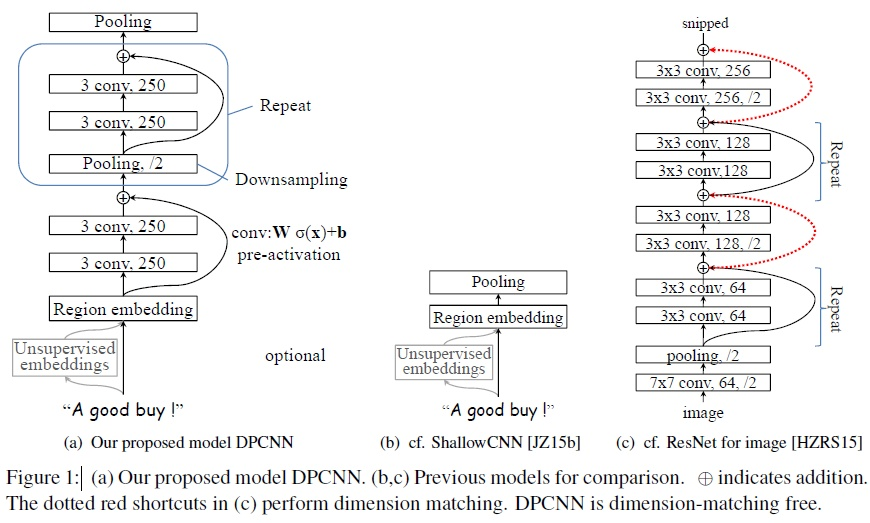
\includegraphics[width=5in, keepaspectratio]{./pic/dpcnn.png}\\
    \caption{DPCNN结构图}
\end{figure}

图中的Shallow CNN即为上一节中的TextCNN.

\subsection{BiLSTM}

用双向LSTM进行文本分类,取其最后一个时间步上的隐状态过分类器。

在长文本分类情境下,这种做法会损失大量的中间信息,
将极大影响模型的性能。

\begin{figure}[htb]
    \centering
    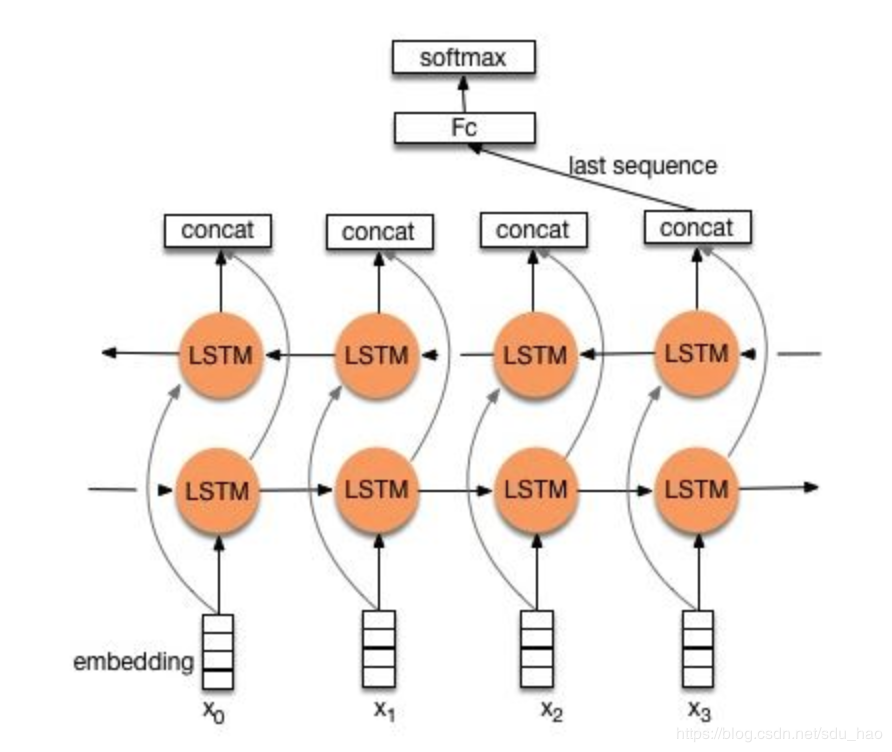
\includegraphics[width=4in, keepaspectratio]{./pic/rnn.png}\\
    \caption{BiLSTM结构图}
\end{figure}

\subsection{BiLSTM with Attention}

在BiLSTM的基础上引入注意力机制:
取双向LSTM所有时间步的隐状态输入Attention层,
取Attention层的输出作为文本的特征表示。

Attention机制大大增强了RNN提取全局信息的能力,
但损失了语序关系。

\begin{figure}[htb]
    \centering
    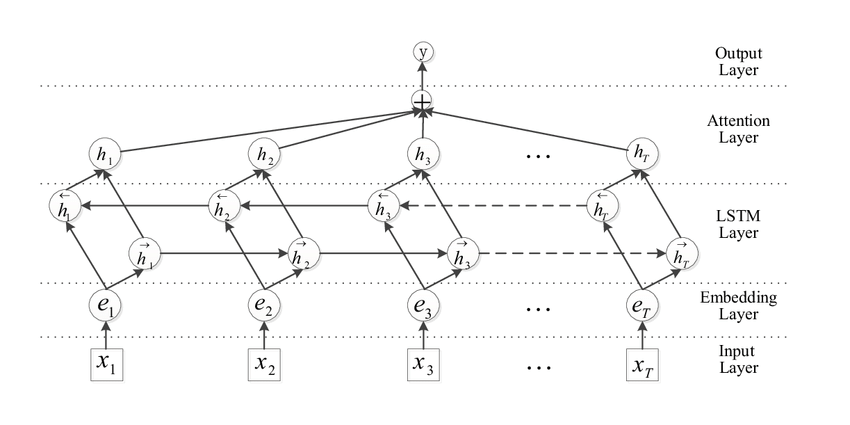
\includegraphics[width=5in, keepaspectratio]{./pic/attn.png}\\
    \caption{BiLSTM with Attention结构图}
\end{figure}

\subsection{TextRCNN}

TextRCNN
\footnote{\href{http://www.aaai.org/ocs/index.php/AAAI/AAAI15/paper/download/9745/9552}
{[Recurrent Convolutional Neural Networks for Text Classification, 2015]}}
把TextCNN和RNN结合到了一起。它将双向LSTM的输入和输出拼接在一起,
经过激活函数后做max pooling,是基于RNN文本分类的又一种策略。


\begin{figure}[htb]
    \centering
    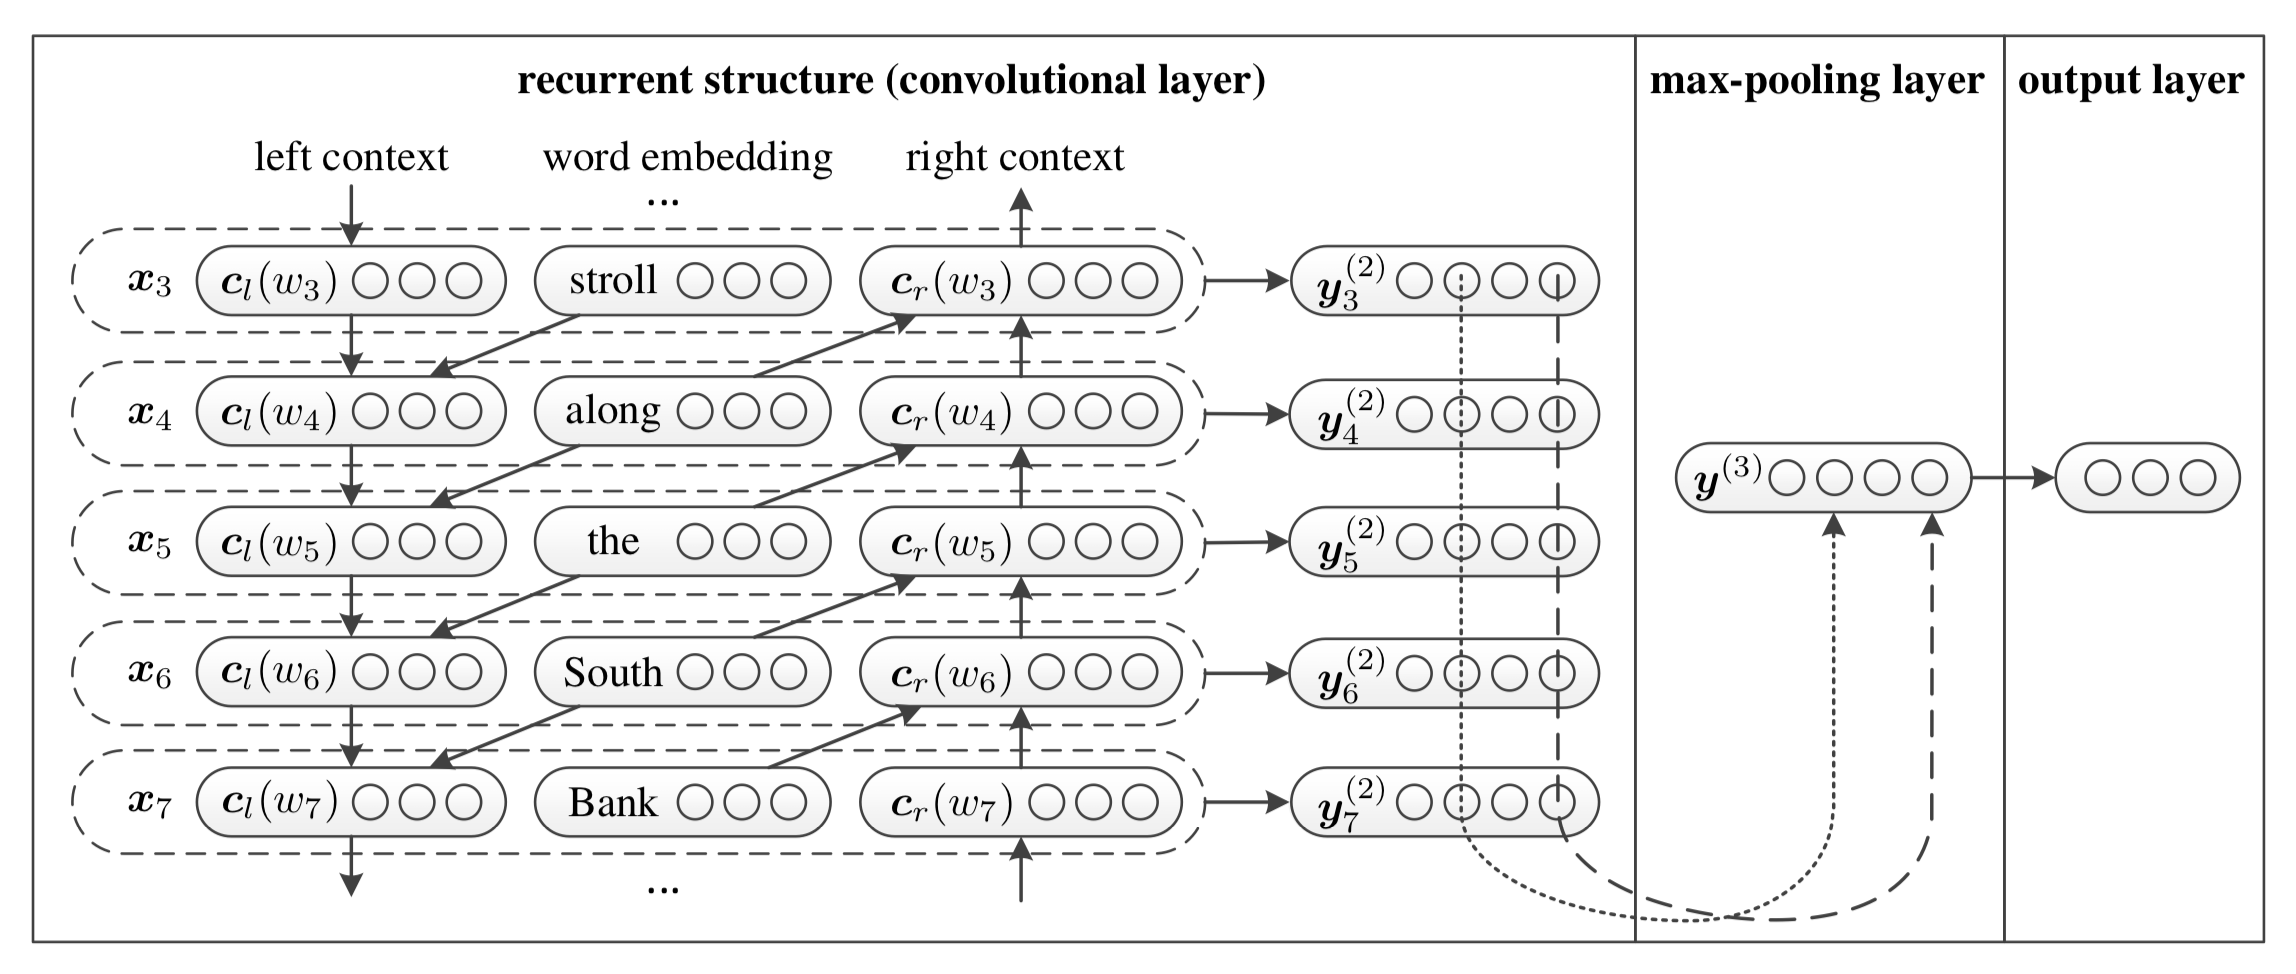
\includegraphics[width=5.6in, keepaspectratio]{./pic/rcnn.png}\\
    \caption{TextRCNN结构图}
\end{figure}


\subsection{BERT}

BERT是基于Transformer的大型预训练网络,代表了NLP领域的state-of-the-art,
仍然是研究的热点。
在本次实验中,我取哈工大发布的RoBERTa-wwm-base前三层,即RBT3
\footnote{https://github.com/ymcui/Chinese-BERT-wwm}
作为特征提取器,在训练集上对其进行微调。

\subsection{TextGCN}

用图卷积网络做文本分类
\footnote{\href{https://arxiv.org/abs/1809.05679}
{[Graph Convolutional Networks for Text Classification, 2019]}},
构建基于文本和词的异构图。

图包含了document和word两类节点,document-word和word-word两种边。
document-word边的权重是TF-IDF,word-word边的权重是通过一种叫PMI的方法计算的。
简单来说,就是统计两个词共现的频率,共现次数越多,权重越大。
$$
w_{ij} =
\begin{cases}
  \text{PMI}(i, j)  & i, j \text{ are words}\\
  \text{TF-IDF}(i, j), & i \text{ is document, }j \text{ is word}\\
  1, & i = j\\
  0, & \text{otherwise}
\end{cases}
$$

GCN的原理就不详述了。

\begin{figure}[htb]
    \centering
    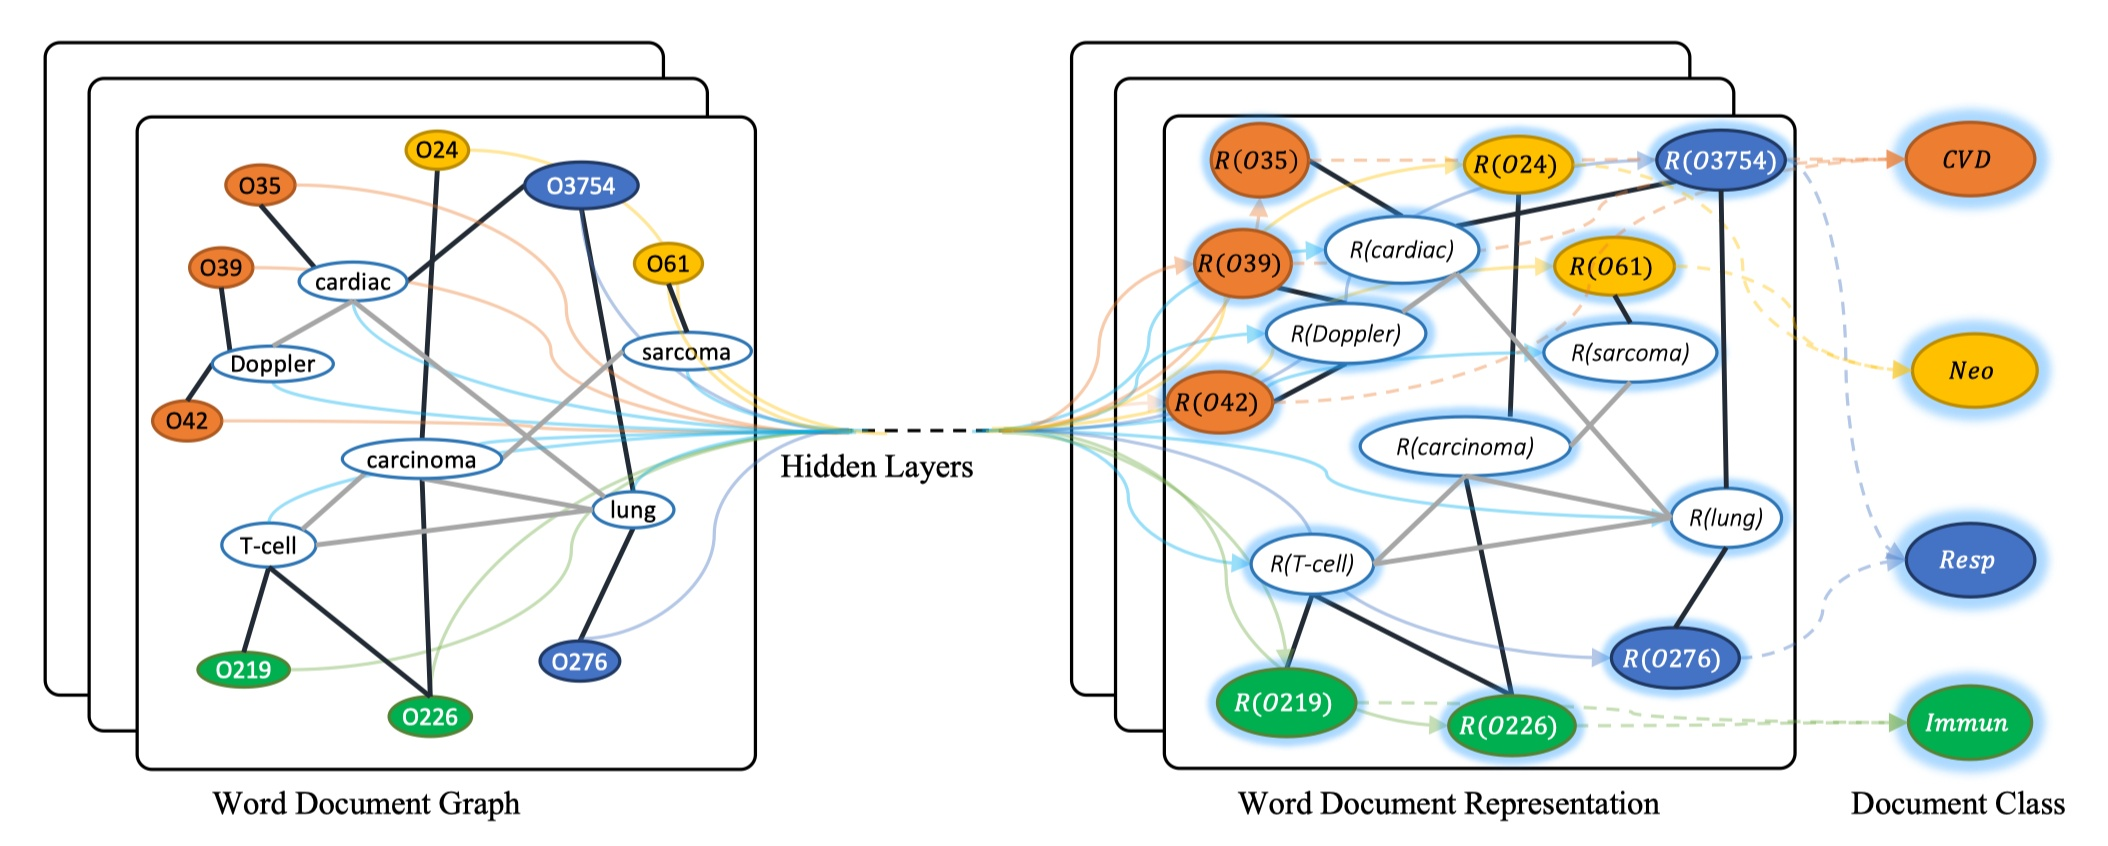
\includegraphics[width=5in, keepaspectratio]{./pic/gcn.jpg}\\
    \caption{TextGCN结构图}
\end{figure}

\section{成果展示}

运行和复现方法见readme文件。

以测试集为准确率为优化指标。测试结果如下。

考虑到对数据集预处理的不同,
各项指标只表示模型性能的相对关系,不应与其它同学的结果相比较。

\begin{table}[htbp]
    \centering
    \caption{各模型测试结果}
\begin{tabular}{lccc}
    \toprule
    Model & Acc & macro F1 & coef \\ 
    \midrule
    Naive Bayes & 61.89\% & 0.2852 & 0.5916 \\ 
    SVM & 60.48\% & 0.2317 & - \\ 
    Random Forest & 59.28\% & 0.1875 & 0.6093 \\ 
    MLP & 59.68\% & 0.2466 & 0.6215 \\ 
    fastText(bow) & 61.79\% & 0.3412 & 0.6309 \\ 
    fastText(bigram) & 63.19\% & 0.3481 & 0.6422 \\ 
    TextCNN & 64.69\% & 0.3362 & \textbf{0.6694} \\ 
    DPCNN & 64.09\% & 0.3371 & 0.6274 \\ 
    BiLSTM & 51.86\% & 0.1222 & 0.4492 \\ 
    BiLSTM with Attention & 62.59\% & 0.3236 & 0.6329 \\
    TextRCNN & \textbf{65.10\%} & 0.3593 & 0.6498 \\ 
    RBT3 & 62.09\% & 0.3490 & 0.6350 \\ 
    TextGCN & 64.69\% & \textbf{0.3647} & -\\
    \bottomrule
    \end{tabular}
\end{table}
\section{实验细节}

选择Adam作为优化器,使用预训练的word2vec词向量进行word embedding,
在本次实验的小样本背景下,固定词向量的效果是最好的。

受篇幅和时间所限,
下文中只展示TextCNN,DPCNN和TextRCNN这三个模型的调参过程,
详细超参数见config文件夹。

\begin{table}[htbp]
    \centering
    \caption{dropout率对TextCNN的影响}
    \begin{tabular}{cccccc}
        \toprule
        dropout率 & 0.1 & 0.3 & 0.5 & 0.7 & 0.9 \\
        \midrule
        Acc & 62.26\% & 63.69\% & \textbf{64.49\%} & 63.99\% & 62.99\% \\
        \bottomrule
    \end{tabular}
\end{table}

dropout的引入使TextCNN的测试准确率提高了两个百分点,效果非常明显。
当dropout率为0.5时模型表现最佳,恰与原论文中作者推荐的超参数相同。

\begin{table}[htbp]
    \centering
    \caption{网络深度对DPCNN的影响}
    \begin{tabular}{cccccccc}
    \toprule
        Layer & 0 & 1 & 2 & 3 & 4 & 6 \\ 
    \midrule
        Acc & 62.99\% &\textbf{64.09\%} & 62.89\% & 63.19\% & 63.09\% & 61.79\% \\ 
    \bottomrule
    \end{tabular}
\end{table}

当DPCNN的池化-卷积-卷积层个数为1时其表现最佳,当网络过深时,模型的表现反而下降。

探究初始化方式及LSTM/GRU对TextRCNN测试集准确率的影响,对比实验如下。

\begin{table}[htbp]
    \centering
    \caption{初始化方式和网络结构对TextRCNN的影响}
    \begin{tabular}{ccccc}
        \toprule
        类型 & 初始化 & Acc  \\ 
        \midrule
        LSTM & 默认 & \textbf{65.10\%}  \\ 
        GRU & 默认 & 64.49\%  \\ 
        LSTM & 正交 & 63.11\% \\ 
        \bottomrule
    \end{tabular}
\end{table}

\FloatBarrier

可见LSTM的效果略优于GRU;
与默认(零均值均匀)初始化方式相比,正交初始化对于提高TextRCNN的性能并无帮助。

\section{思考题}

\textbf{实验训练什么时候停止是最合适的?简要陈述你的实现方式,并试分析
固定迭代次数与通过验证集调整等方法的优缺点。}

固定迭代次数的方法能充分挖掘模型的潜能,但会浪费计算资源,
适合在模型较小或计算资源充足时使用。

通过验证集调整,即在验证集性能长期不提升时终止训练,能够节省计算资源,
但可能错失最佳模型。

考虑到本次实验无论是数据量还是模型都比较小,
我选用固定迭代次数的方式,
选取在验证集上表现最好的模型进行最终测试。\\

\textbf{实验参数的初始化是怎么做的?不同的方法适合哪些地方?
(均匀分布初始化,高斯分布初始化,正交初始化等)}

用PyTorch默认的初始化方式。

具体而言,全连接层、卷积层、LSTM用零均值均匀分布初始化;
Batch Normalization初始化权重采样于$U(0,1)$, 偏置初始化为0。

正交初始化是为了解决梯度消失和梯度爆炸的问题设计的,适用于RNN,
但在本次实验中并没有帮助。

我认为各种初始化方法的应用是case by case的,
应当通过实验确定哪一种方法更好。\\

\textbf{过拟合是深度学习常见的问题,有什么方法可以方式训练过程陷入过拟
合?}

\begin{itemize}
    \item Early Stoping:在模型过拟合之前及时停止训练;
    \item Dropout:前向传播时,让神经元以一定的概率停止工作,
    使模型不会过度依赖局部特征,从而增强其泛化能力;
    \item L2(L1)-penalty:限制参数的范数以防止模型过于复杂;
    \item 数据增强或增加训练数据:最有效的方法,但不一定可行;
    \item 各种normalization往往也有一定的正则化效果。
\end{itemize}

\textbf{试分析CNN,RNN,MLP三者的优缺点。}

MLP:作为词袋模型,MLP不能有效利用上下文信息,但它结构简单,训练速度快。
fastText就是其中的佼佼者,效果也算中规中矩。

CNN:卷积层参数量小,不易过拟合,能够有效提取局部的语义信息。
缺点是难以捕捉长距离依赖关系,但在本实验背景下,
这个问题造成的影响不大。

RNN:能更好的处理长距离依赖,配合Attention机制具备有限的可解释性,
也容易处理变长序列。
缺点是并行度低,训练耗时长,存在梯度消失和梯度爆炸的问题,也不擅长提取局部语义信息。

\section{总结反思}

在本次实验中,我用sklearn和PyTorch搭建了各种经典的情感分类模型,
对它们的特点和优劣有了更深的认识,花费了相当大的精力,确实也有所收获。

神经网络的模型设计是非常自由的,比如Attention层不仅可以接在LSTM的后面,
还可以用在卷积层之前,这也是提高卷积层提取全局特征能力的一个idea。

\end{document}